%%%%%%%%%%%%%%%%%%%%%%%%%%%
% PROBABILISTIC INVERSION %
%%%%%%%%%%%%%%%%%%%%%%%%%%%
We begin with Bayesian probabilistic inversion, on the basis of which we demonstrate how one can quantify the material variability within the ensemble of beams in a series of bending tests.
A numerical experiment is therefore set up as follows.
% EXPERIMENTAL SETUP
We consider a number of \(n=100\) beams with well-known dimensions \(L_i=\unit[1]{m}\) and \(b_i=h_i=\unit[10]{cm}\).
Beams are subjected to concentrated loads \(F_i=\unit[30]{kN}\) that are applied at midspan.
For \(i=1,\ldots,100\) Young's moduli \(E_i\) are independently sampled from a lognormal distribution \(\mathcal{LN}(E_i \cond \mu_E,\sigma_E)\) with mean \(\mu_E=\unit[15]{GPa}\) and standard deviation \(\sigma_E=\unit[3]{GPa}\).
This corresponds to a coefficient of variation \(c_{E} = \unit[20]{\%}\).
% TREATED AS UNKNOWNS
After having set up the experiment, the hyperparameters \(\bm{\theta}_E=(\mu_E,\sigma_E)\) as well as beam-specific moduli \(E_i\) will be treated as unknowns. 
% PREDICTED DEFLECTIONS
At \(n_i=3\) positions \(\bm{s}_i = (s_{i,1},s_{i,2},s_{i,3})\) with \(s_{i,1}=\unit[25]{cm}\), \(s_{i,2}=\unit[50]{cm}\) and \(s_{i,3}=\unit[75]{cm}\)
beam deflections \(\perfect{\bm{v}}_i = (\perfect{v}_i(s_{i,1}),\perfect{v}_i(s_{i,2}),\perfect{v}_i(s_{i,3}))\) are computed according to \cref{eq:PEM:Beams:AlgebraicFormula}.
% MEASUREMENT UNCERTAINTY
In order to take measurement uncertainty and forward model imperfection into account, we perturb the predictions \(\perfect{\bm{v}}_i\) with noise terms \(\bm{\varepsilon}_i = (\varepsilon_{i,1},\varepsilon_{i,2},\varepsilon_{i,3})\).
Those terms are independently sampled from Gaussian distributions \(\mathcal{N}(\bm{\varepsilon}_i \distparam \bm{0},\bm{\Sigma}_i)\) with \(\bm{\Sigma}_i = \sigma_i^2 \bm{I}_3\) and \(\sigma_i = \unit[0.1]{mm}\).
% PSEUDO DATA & INFERENTIAL GOAL
Eventually \(\bm{v}_i = \perfect{\bm{v}}_i + \bm{\varepsilon}_i\) represent the pseudo data that will become analyzed with respect to the QoI \(\bm{\theta}_E = (\mu_E,\sigma_E)\).
\par % HYPERPRIOR MODEL
In many circumstances expert knowledge about the QoI \(\bm{\theta}_E\) is available prior to analyzing the data.
This knowledge can be accounted for by eliciting a suitable prior distribution \(\pi(\bm{\theta}_E)\).
Herein we employ a proper Bayesian prior \(\pi(\bm{\theta}_E) = \pi(\mu_E) \, \pi(\sigma_E)\) with independent marginals.
As measured in units of \(\unit[]{GPa}\) those marginals are given as uniform distributions \(\pi(\mu_E) = \mathcal{U}(0,100)\) and \(\pi(\sigma_E) = \mathcal{U}(0,30)\).
This is supposed to represent an experimental situation where one cannot elicit informative priors, nonetheless one is confident enough to assign this weakly informative and flat prior with its upper and lower bounds.
\par % PROBABILISTIC INVERSION
Ultimately probabilistic inversion can be summarized as the estimation of the QoI \(\bm{\theta}_{\bm{X}} \equiv \bm{\theta}_E\) with the deflection measurements \(\tuple{\bm{y}_i} \equiv \tuple{\bm{v}_i}\).
Beam-specific Young's moduli \(\tuple{\bm{x}_i} \equiv \tuple{E_i}\), that are not of immediate inferential interest, are considered nuisance to that end.
Experimental conditions \(\tuple{\bm{d}_i} \equiv \tuple{(F_i,\bm{l}_i,\bm{s}_i)}\), that the experiments where subject to, and prediction error models \(\tuple{\bm{\Sigma}_i}\) are assumed to be known.
The distributions \(f_{\bm{X} \cond \bm{\Theta}_{\bm{X}}} (\bm{x}_i \cond \bm{\theta}_{\bm{X}}) \equiv \mathcal{LN}(E_i \cond \mu_E,\sigma_E)\) and
\(\pi_{\bm{\Theta}_{\bm{X}}}(\bm{\theta}_{\bm{X}}) \equiv \pi(\bm{\theta}_E)\) represent the available structural and parametric prior knowledge, respectively.
The emerging posterior will be of the form \(\pi( \bm{\theta}_{\bm{X}} \cond \tuple{\bm{y}_i}) \equiv \pi( \bm{\theta}_E \cond \tuple{\bm{v}_i})\).
It can be directly sampled or accessed via the QoI-marginals of the joint posterior \(\pi( \tuple{\bm{x}_i},\bm{\theta}_{\bm{X}} \cond \tuple{\bm{y}_i}) \equiv \pi( \tuple{E_i},\bm{\theta}_E \cond \tuple{\bm{v}_i})\).
% DAG
A DAG corresponding to probabilistic inversion is provided in \cref{fig:PEM:DAG:ProbInv}.

\subsubsection{MCMC}
% JOINT VS. MARGINAL
Generally we employ a joint rather than a marginal problem formulation.
% EXACT POSTERIOR SAMPLING
For the fidelity reasons that were discussed in \cref{sec:PEM:Computations:MultilevelChallenges} this allows for exact posterior computation where an approximation is only introduced in as much as MCMC sampling is concerned.
% ADDITIONAL INSIGHT
Moreover a joint posterior features a richer structure which will provide new insights into multilevel inversion.
% COMPUTER ISSUES
All computations will be serially done on a contemporary Intel Xeon CPU.
\par % MCMC
The joint posterior \(\pi(\tuple{E_i},\bm{\theta}_E \cond \tuple{\bm{v}_i})\) is sampled by means of a blockwise random walk Metropolis algorithm.
% CUMBERSUME TUNING
A practical problem of random walk samplers in high dimension is to carefully tune the proposal distribution.
For complex multivariate posterior distributions this is a cumbersome procedure that poses severe difficulties.
% SYMMETRY CONSIDERATIONS
However, in multilevel inversion one can advantageously exploit the ``symmetry'' of the problem in the latent variables.
Assuming that separate inverse problems \(i\) with \(1 \leq i \leq n\) are not severely ill-posed, latent variables of the same uncertainty type are expected to behave similarly in the sense that their marginal posteriors resemble one another.
Moreover, due to the indirectness of borrowing strength, their mutual correlations are expected to be rather small.
Along these lines the ``effective dimensionality'' is lower than the number of unknowns suggests.
% BLOCKWISE STRUCTURE
This discussion motivates that MCMC updates are done in blocks \(\tuple{E_i}\) and \((\mu_E,\sigma_E)\).
% ACCEPTANCE RATES
We find that with Gaussian jumping distributions the algorithm can be easily tuned in such a way that blockwise acceptance rates range between \(\unit[20]{\%}\) and \(\unit[40]{\%}\).
% INITIALIZATION
Avoiding lengthy convergence times in high-dimensional problems requires smart initialization, too.
Again we proceed by exploiting the structure of the multilevel system.
The block \(\tuple{E_i}\) is initialized with solutions of separate inverse problems, while two-stage estimates are used in the hyperparameter block \((\mu_E,\sigma_E)\).
\par % CONVERGENCE
In order to assure duly completed posterior exploration we perform a number of convergence checks.
The algorithm is initialized in regions of the parameter space that had not been visited before and the convergence behavior of the Markov chain is monitored.
We detect that the chain eventually reaches the same posterior modes again.
% TRACE PLOTS
In \cref{fig:PEM:ProbInv:Chains} trace plots of a converging Markov chain are shown for its \(\mu_E\) and \(\sigma_E\) components.
They have been initialized at \(\mu_E^{(0)}=\unit[50]{GPa}\) and \(\sigma_E^{(0)}=\unit[15]{GPa}\), i.e.\ in the middle of their priorly admissible intervals.
% CONVERGENCE BEHAVIOR
While the mean hyperparameter \(\mu_E\) directly converges as shown in \cref{fig:PEM:ProbInv:Chain:Mean}, we observe a different behavior for the spread hyperparameter \(\sigma_E\).
From \cref{fig:PEM:ProbInv:Chain:Sigma} it can be seen that the latter chain tends to higher values prior to attraction towards the posterior mean.
% INTERPRETATION
For the given initialization this is a systematic effect that indicates a posterior correlation in the hyperparameters \((\mu_E,\sigma_E)\).
Eventually the Markov chain converges within ca.\ \(400\) MCMC iterations.
% ADVANCED DIAGNOSTICS
Apart from such visual inspections we generally rely on Gelman-Rubin diagnostics for parallel chains \cite{MCMC:Gelman1992,MCMC:Brooks1998:Gelman}.
% MARKOV CHAINS
\begin{figure}[ht]
  \centering
  \begin{subfigure}[b]{0.5\textwidth}
    \centering
    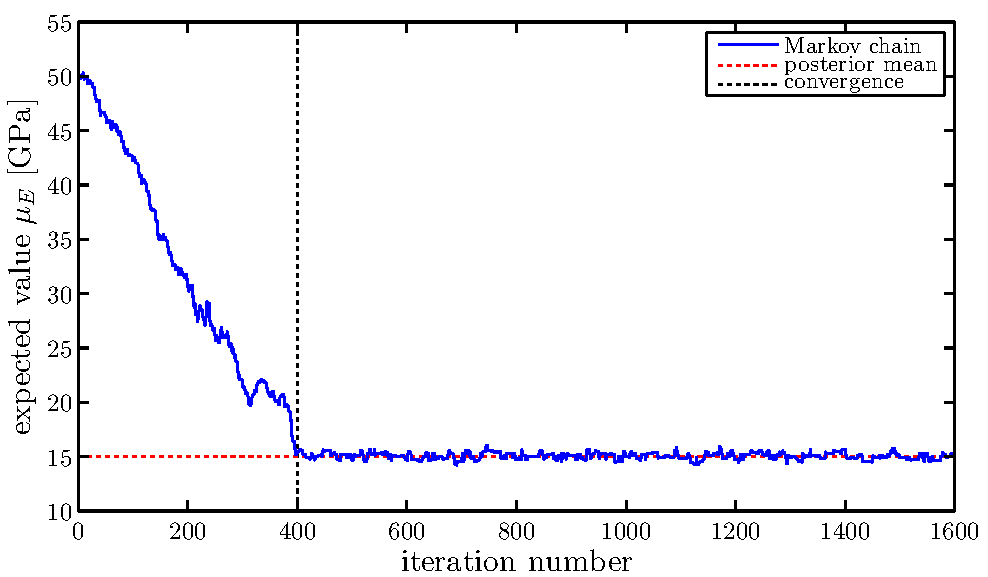
\includegraphics[height=\PEMfigHeight]{fig_PEM_ProbInvChainMean}
    \caption{Convergence of \(\mu_E\).}
    \label{fig:PEM:ProbInv:Chain:Mean}
  \end{subfigure}%
  \begin{subfigure}[b]{0.5\textwidth}
    \centering
    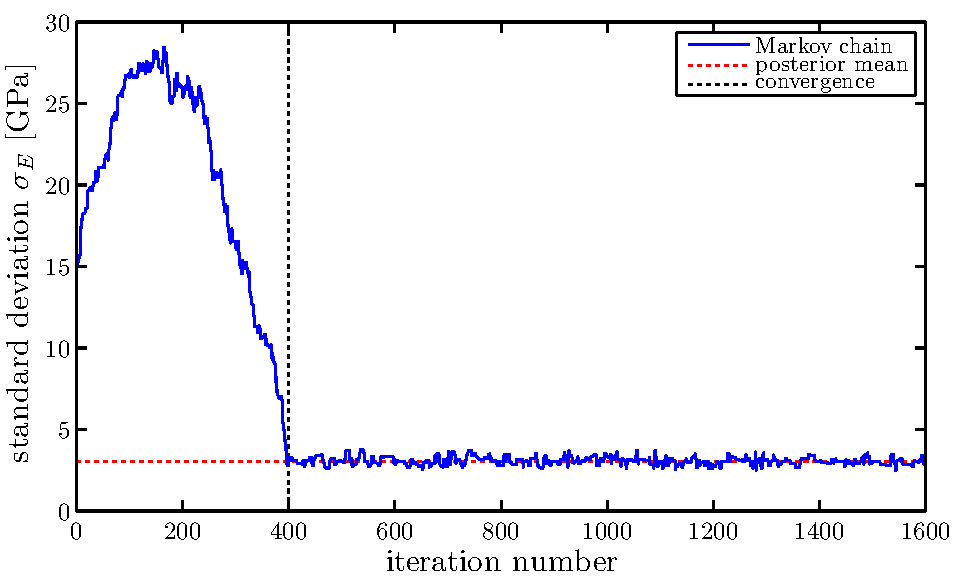
\includegraphics[height=\PEMfigHeight]{fig_PEM_ProbInvChainSigma}
    \caption{Convergence of \(\sigma_E\).}
    \label{fig:PEM:ProbInv:Chain:Sigma}
  \end{subfigure}%
  \caption[Trace plots of a converging Markov chain]{Trace plots of a converging Markov chain.
           For \(n=100\) the converging Markov chain is shown for \(\mu_E\) in \subref{fig:PEM:ProbInv:Chain:Mean} and for \(\sigma_E\) in \subref{fig:PEM:ProbInv:Chain:Sigma}.
           Being initialized at \(\mu_E^{(0)}=\unit[50]{GPa}\) and \(\sigma_E^{(0)}=\unit[15]{GPa}\) the Markov chain converges within ca.\ \(400\) MCMC iterations.
           In equilibrium the Markov chain samples the posterior around its mean.
           }
  \label{fig:PEM:ProbInv:Chains}
\end{figure}
\par % AUTOCORRELATION
In \cref{fig:PEM:ProbInv:ACF} the MCMC sample autocorrelations are plotted for the QoI \((\mu_E,\sigma_E)\) and for an intermediate variable \(E_i\) with \(i=1\).
It can be seen how the autocorrelation function (ACF) drops until it becomes indistinguishable from zero.
This behavior governs the quality of the sample as a posterior representative.
Especially the ACF of \(E_i\) shown in \cref{fig:PEM:ProbInv:ACF:Param} motivates more efficient updating schemes in future research.
% AUTOCORRELATION
\begin{figure}[ht]
  \centering
  % MEAN HYPERPARAMETER
  \begin{subfigure}[b]{0.33\textwidth}
    \centering
    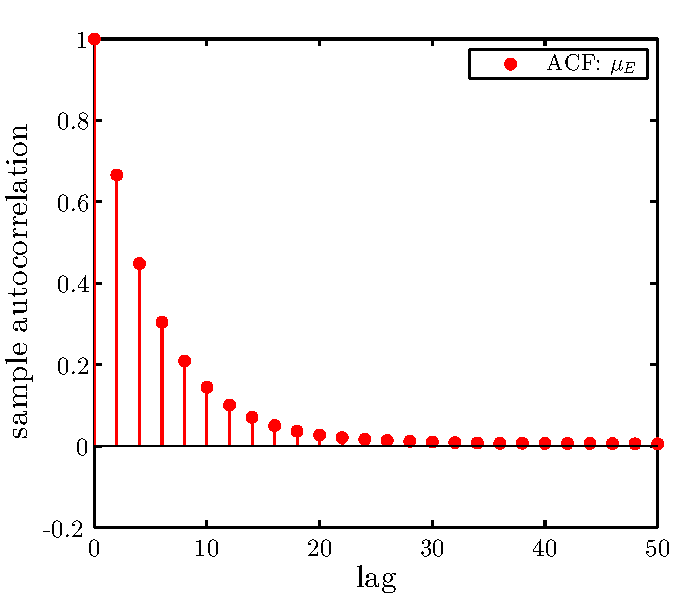
\includegraphics[height=\PEMfigHeight]{fig_PEM_ProbInvACFMean}
    \caption{Autocorrelation of \(\mu_E\).}
    \label{fig:PEM:ProbInv:ACF:Mean}
  \end{subfigure}%
  % SIGMA HYPERPARAMETER
  \begin{subfigure}[b]{0.33\textwidth}
    \centering
    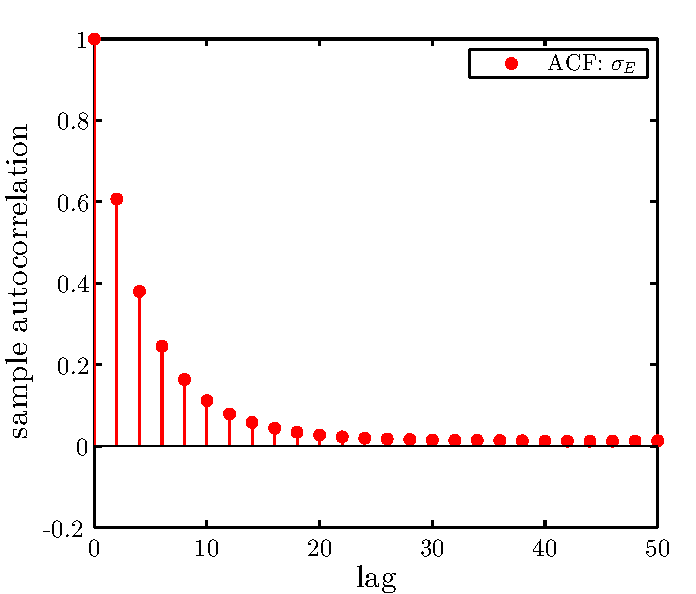
\includegraphics[height=\PEMfigHeight]{fig_PEM_ProbInvACFSigma}
    \caption{Autocorrelation of \(\sigma_E\).}
    \label{fig:PEM:ProbInv:ACF:Sigma}
  \end{subfigure}%
  % INDIVIDUAL PARAMETER
  \begin{subfigure}[b]{0.33\textwidth}
    \centering
    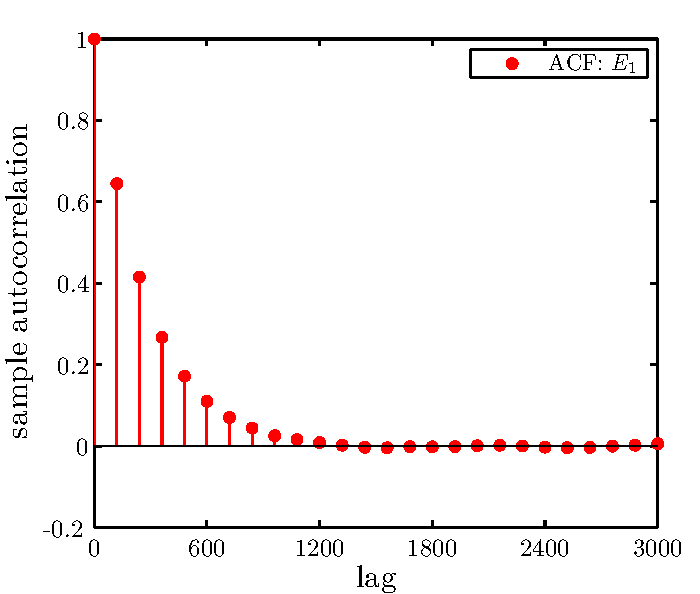
\includegraphics[height=\PEMfigHeight]{fig_PEM_ProbInvACFParam}
    \caption{Autocorrelation of \(E_1\).}
    \label{fig:PEM:ProbInv:ACF:Param}
  \end{subfigure}%
  \caption[Sample autocorrelation functions]{Sample autocorrelation functions.
           For a run with \(n=100\) the MCMC sample autocorrelation function is plotted for \(\mu_E\) in \subref{fig:PEM:ProbInv:ACF:Mean},
           for \(\sigma_E\) in \subref{fig:PEM:ProbInv:ACF:Sigma} and for \(E_1\) in \subref{fig:PEM:ProbInv:ACF:Param}.
           The sample autocorrelation determines the effective MCMC sample size.
           }
  \label{fig:PEM:ProbInv:ACF}
\end{figure}

\subsubsection{Results: Posterior marginals}
% ANALYZED DATA
We analyze the data \(\tuple{\bm{v}_i}_{1\leq i \leq 100}\) as well as its subconfigurations \(\tuple{\bm{v}_i}_{1 \leq i \leq 10}\), \(\tuple{\bm{v}_i}_{1\leq i \leq 20}\) and \(\tuple{\bm{v}_i}_{1\leq i \leq 50}\).
This allows to assess how the number of experiments \(n\) influences the identification of the QoI.
% MCMC ITERATIONS
For each of the runs \(N=10^7\) MCMC iterations are performed.
% BURN-IN
As a general rule we discard the initial \(\unit{1}{\%}\) of the total number of iterations of each Markov chain as a burn-in period.
% COMPUTATION TIME
The total algorithm runtime adds up to \(t=\unit[3.85]{h}\) for \(n=10\) and to \(t=\unit[4.66]{h}\) for \(n=100\).
% POSTERIOR MARGINALS
The resulting posterior marginals of \(\mu_E\) and \(\sigma_E\) are shown in \cref{fig:PEM:ProbInv:Marginals}.
% TABLE
A statistical summary of these marginals can be found in \cref{tab:PEM:ProbInf:Summary}, where the mean, mode, standard deviation (SD) and coefficient of variation (CV) are listed.
% REMARKS
With increasing number of processed experiments \(n\),
Bayesian point estimates (mean, mode) approach the true values \(\mu_E = \unit[15]{GPa}\) and \(\sigma_E = \unit[3]{GPa}\) while measures of estimation uncertainty (SD, CV) expectedly decrease.
% MARGINAL POSTERIORS
\begin{figure}[ht]
  \centering
  \begin{subfigure}[b]{0.5\textwidth}
    \centering
    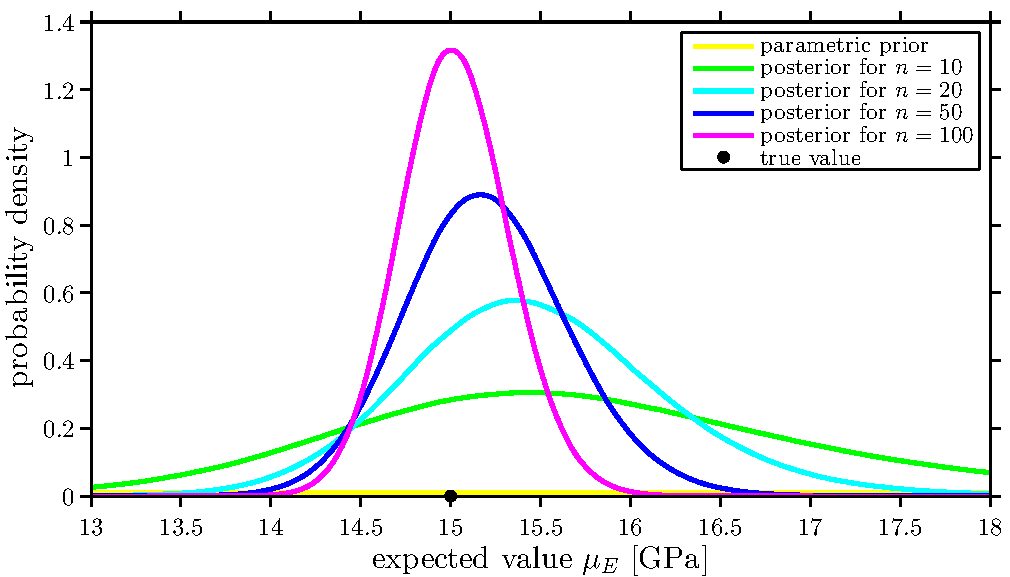
\includegraphics[height=\PEMfigHeight]{fig_PEM_ProbInvPostMean}
    \caption{Posterior marginal of \(\mu_E\).}
    \label{fig:PEM:ProbInv:Post:Mean}
  \end{subfigure}%
  \begin{subfigure}[b]{0.5\textwidth}
    \centering
    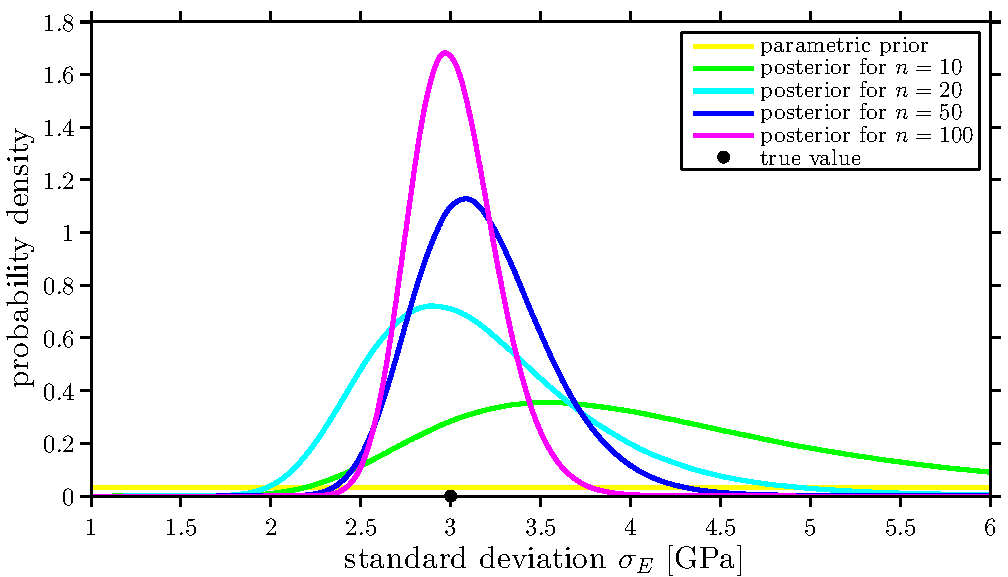
\includegraphics[height=\PEMfigHeight]{fig_PEM_ProbInvPostSigma}
    \caption{Posterior marginal of \(\sigma_E\).}
    \label{fig:PEM:ProbInv:Post:Sigma}
  \end{subfigure}%
  \caption[Posterior marginals of the QoI]{Posterior marginals of the QoI.
           Corresponding to various numbers of experiments \(n\), the marginal posterior densities of \(\mu_E\) and \(\sigma_E\)
           are shown in \subref{fig:PEM:ProbInv:Post:Mean} and \subref{fig:PEM:ProbInv:Post:Sigma}, respectively.
           For increasing \(n\), the posterior uncertainty in estimating the QoI \(\bm{\theta}_E = (\mu_E,\sigma_E)\)
           with \(\mu_E=\unit[15]{GPa}\) and \(\sigma_E = \unit[3]{GPa}\) steadily decreases.
          }
  \label{fig:PEM:ProbInv:Marginals}
\end{figure}
% TABLE: PROBABILISTIC INVERSION
\begin{table}[ht]
  \caption[Summary of the QoI posterior marginals]{Summary of the QoI posterior marginals.}
  \label{tab:PEM:ProbInf:Summary}
  \centering
  \begin{tabular}{lcccccccccc}
    \toprule
    & \phantom{} & \multicolumn{3}{c}{\(\mu_E\) \(\lbrack\unit[]{GPa}\rbrack\)} & \(\lbrack \unitless \rbrack\)
    & \phantom{} & \multicolumn{3}{c}{\(\sigma_E\) \(\lbrack\unit[]{GPa}\rbrack\)} & \(\lbrack \unitless \rbrack\) \\
    \cmidrule{3-6} \cmidrule{8-11}
    && Mean & Mode & SD & CV && Mean & Mode & SD & CV \\
    \midrule
    \(n=10\)  && \(15.98\) & \(15.43\) & \(2.06\) & \(0.13\) && \(4.73\) & \(3.54\) & \(3.55\) & \(0.75\) \\
    \(n=20\)  && \(15.48\) & \(15.36\) & \(0.74\) & \(0.05\) && \(3.18\) & \(2.90\) & \(0.65\) & \(0.20\) \\
    \(n=50\)  && \(15.20\) & \(15.17\) & \(0.46\) & \(0.03\) && \(3.17\) & \(3.08\) & \(0.37\) & \(0.12\) \\
    \(n=100\) && \(15.02\) & \(15.00\) & \(0.30\) & \(0.02\) && \(3.02\) & \(2.97\) & \(0.24\) & \(0.08\) \\
    \bottomrule
  \end{tabular}
\end{table}

\subsubsection{Results: Two-dimensional posteriors}
% 2D POSTERIOR
Showing posterior marginals may hide possibly existing dependency structures or the lack thereof.
Those constitute a substantial result of Bayesian data analysis, though.
Hence \cref{fig:PEM:ProbInv:2DPosterior} shows two-dimensional posteriors where interesting correlation properties were discovered.
% HYPERPARAMETERS
The two-dimensional posterior of \((\mu_E,\sigma_E)\) is plotted in \cref{fig:PEM:ProbInv:2DPosterior:MeanSigma}.
According to the posterior probability model these two parameters are correlated with a linear Pearson coefficient of correlation \(r_{\mu_E,\sigma_E}=0.40\).
Note that these parameters were assumed to be independent in accord with their prior model.
% JOINT POSTERIOR
The joint posterior \cref{eq:PEM:ProbInv:JointPosterior} can also feature a correlation between hyperparameters and experiment-specific parameters.
In \cref{fig:PEM:ProbInv:2DPosterior:MeanParam,fig:PEM:ProbInv:2DPosterior:ParamParam} the two-dimensional posteriors of \((\mu_E,E_i)\) and \((E_{j},E_{i})\) with \(i=50\) and \(j=75\) are imaged.
% 2D POSTERIORS
\begin{figure}[ht]
  \centering
  \begin{subfigure}[b]{0.33\textwidth}
    \centering
    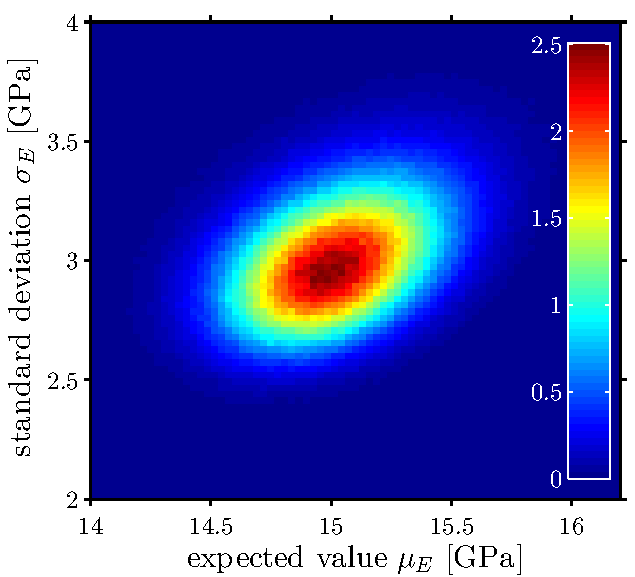
\includegraphics[height=\PEMfigHeight]{fig_PEM_ProbInvPost2DMeanSigma}
    \caption{2D posterior of \((\mu_E,\sigma_E)\).}
    \label{fig:PEM:ProbInv:2DPosterior:MeanSigma}
  \end{subfigure}%
  \begin{subfigure}[b]{0.33\textwidth}
    \centering
    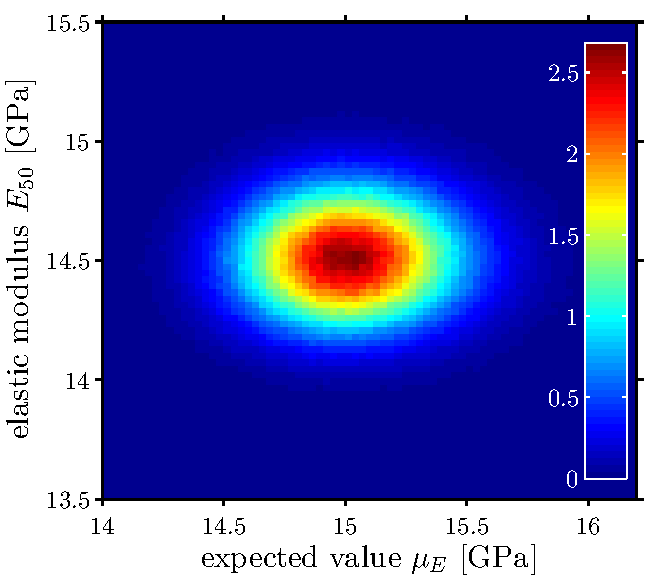
\includegraphics[height=\PEMfigHeight]{fig_PEM_ProbInvPost2DMeanParam}
    \caption{2D posterior of \((\mu_E,E_{50})\).}
    \label{fig:PEM:ProbInv:2DPosterior:MeanParam}
  \end{subfigure}%
  \begin{subfigure}[b]{0.33\textwidth}
    \centering
    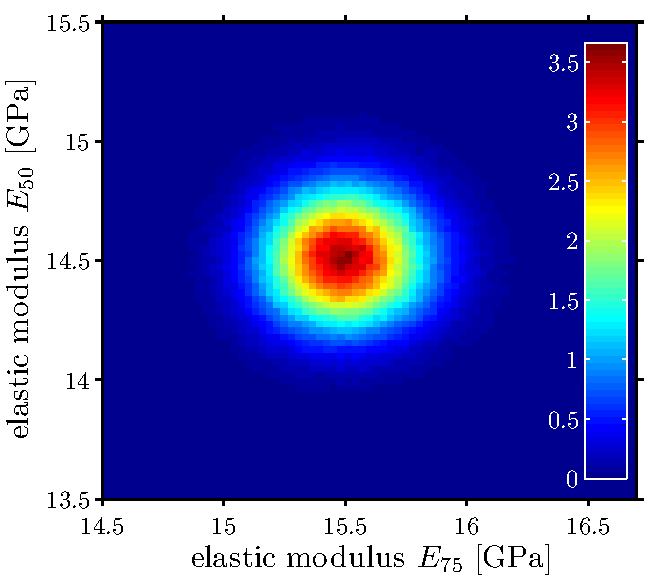
\includegraphics[height=\PEMfigHeight]{fig_PEM_ProbInvPost2DParamParam}
    \caption{2D posterior of \((E_{75},E_{50})\).}
    \label{fig:PEM:ProbInv:2DPosterior:ParamParam}
  \end{subfigure}%
  \caption[2D posteriors of \((\mu_E,\sigma_E)\), \((\mu_E,E_{50})\) and \((E_{75},E_{50})\)]{2D posteriors of \((\mu_E,\sigma_E)\), \((\mu_E,E_{50})\) and \((E_{75},E_{50})\).
           The two-dimensional posteriors of \((\mu_E,\sigma_E)\), \((\mu_E,E_{50})\) and \((E_{75},E_{50})\) are shown.
           Being priorly independent the components \(\mu_E\) and \(\sigma_E\) are seen to be correlated a posteriori.
           The linear Pearson coefficient of correlation amounts to \(r_{\mu_E,\sigma_E}=0.40\).
           }
  \label{fig:PEM:ProbInv:2DPosterior}
\end{figure}